\documentclass[12pt]{beamer}
\usepackage{../Estilos/BeamerMAF}
\usetheme{Dresden}
\usecolortheme{seahorse}
%\useoutertheme{default}
\setbeamercovered{invisible}
% or whatever (possibly just delete it)
\setbeamertemplate{section in toc}[sections numbered]
\setbeamertemplate{subsection in toc}[subsections numbered]
\setbeamertemplate{subsection in toc}{\leavevmode\leftskip=3.2em\rlap{\hskip-2em\inserttocsectionnumber.\inserttocsubsectionnumber}\inserttocsubsection\par}
\setbeamercolor{section in toc}{fg=blue}
\setbeamercolor{subsection in toc}{fg=blue}
\setbeamercolor{frametitle}{fg=blue}
\setbeamertemplate{caption}[numbered]

\setbeamertemplate{footline}
\beamertemplatenavigationsymbolsempty
\setbeamertemplate{headline}{}

\makeatletter
\setbeamercolor{section in foot}{bg=gray!30, fg=black!90!orange}
\setbeamercolor{subsection in foot}{bg=blue!30!yellow, fg=red}
\setbeamertemplate{footline}
{
  \leavevmode%
  \hbox{%
  \begin{beamercolorbox}[wd=.333333\paperwidth,ht=2.25ex,dp=1ex,center]{section in foot}%
    \usebeamerfont{section in foot} \insertsection
  \end{beamercolorbox}}%
  \begin{beamercolorbox}[wd=.333333\paperwidth,ht=2.25ex,dp=1ex,center]{subsection in foot}%
    \usebeamerfont{subsection in foot}  \insertsubsection
  \end{beamercolorbox}%
  \begin{beamercolorbox}[wd=.333333\paperwidth,ht=2.25ex,dp=1ex,right]{date in head/foot}%
    \usebeamerfont{date in head/foot} \insertshortdate{} \hspace*{2em}
    \insertframenumber{} / \inserttotalframenumber \hspace*{2ex} 
  \end{beamercolorbox}}%
  \vskip0pt%
\makeatother 

\makeatletter
\patchcmd{\beamer@sectionintoc}{\vskip1.5em}{\vskip0.8em}{}{}
\makeatother


\date{5 de noviembre de 2021}

\title{\large{Ortogonalización Gram-Schmidt}}
\subtitle{Polinomios de Chebyshev Tipo II}
\author{M. en C. Gustavo Contreras Mayén}

\begin{document}
\maketitle
\fontsize{14}{14}\selectfont
\spanishdecimal{.}

\section*{Contenido}
\frame{\tableofcontents[currentsection, hideallsubsections]}

\section{Ejercicio}
\frame{\tableofcontents[currentsection, hideothersubsections]}
\subsection{Enunciado}

\begin{frame}
\frametitle{Enunciado del problema}
Con el método de ortogonalización de Gram-Schmidt construye los primeros tres polinomios de Chebyshev de Tipo II.
\end{frame}
\begin{frame}
\frametitle{Elementos para el procedimiento}
Considera lo siguiente:
\begin{eqnarray*}
\begin{aligned}
u_{n}(x) &= x^{n} \\[0.5em] \pause
n &= 0, 1, 2, \ldots \\[0.5em] \pause
-1 &\leq x \leq 1 \\[0.5em] \pause
\omega (x) &= (1 -x^{2})^{\frac{1}{2}}
\end{aligned}
\label{eq:}
\end{eqnarray*}
\end{frame}

\subsection{Normalización}

\begin{frame}
\frametitle{Normalización de los polinomios de Chebyshev}
La normalización de los polinomios de Chebyshev de tipo II $U_{n}(x)$, está dada por la expresión:
\pause
\begin{align*}
\scaleint{6ex}_{\bs -1}^{1} \, U_{m}(x) \, U_{n} (x) \, \omega (x) \dd{x} = \delta_{mn} \, \dfrac{\pi}{2}
\end{align*}
\end{frame}

\subsection*{Integral de apoyo}

\begin{frame}
\frametitle{Integral de apoyo}
Para reducir el tiempo en el cálculo de algunas integrales, nos apoyaremos con el siguiente resultado:
\pause
\begin{align*}
\scaleint{6ex}_{\bs -1}^{1} &x^{2n} (1 {-} x^{2})^{\frac{1}{2}} {=} \\[0.5em]
&= \begin{cases}
\dfrac{\pi}{2} \, \dfrac{1 \cdot 3 \cdot 5 \cdots (2 \, n {-} 1)}{4 \cdot 6 \cdot 8 \cdots (2 \, n {+} 2)} & n {=} 1, 2, \ldots \\[1em]
\dfrac{\pi}{2} & n {=} 0
\end{cases}
\end{align*}
\end{frame}

\section{Cambiando el valor de \texorpdfstring{$n$}{n}}
\frame{\tableofcontents[currentsection, hideothersubsections]}
\subsection{Caso \texorpdfstring{$n=0$}{n=0}}

\begin{frame}
\frametitle{Comenzando con el procedimiento}
Al seguir la técnica de ortogonalización, \pause tomamos $n = 0$:
\pause
\begin{eqnarray*}
\begin{aligned}
&\Rightarrow u_{0} (x) = 1 \pause \hspace{1cm} \psi_{0}(x) =  1 \\[0.5em] \pause
&\Rightarrow \varphi_{0}(x) = \dfrac{N_{0} \, \psi_{0}}{\bigg[ \scaleint{6ex} \big[ \psi_{0} \big]^{2} \omega \dd{x} \bigg]^{\frac{1}{2}}} = \\[0.5em] \pause
&N_{0}^{2} = \dfrac{\pi}{2}
\end{aligned}
\end{eqnarray*}
\end{frame}
\begin{frame}
\frametitle{Resolviendo las operaciones}
La integral del denominador resulta:
\pause
\begin{eqnarray*}
\begin{aligned}
\bigg[ \scaleint{6ex}_{\bs -1}^{1} (&1 - x^{2})^{\frac{1}{2}} \bigg]^{\frac{1}{2}} = \pause \bigg[ \dfrac{\pi}{2} \bigg]^{\frac{1}{2}} \\[0.5em] \pause
&\Rightarrow \varphi_{0}(x) = \dfrac{N_{0} \, \psi_{0}}{\bigg[ \scaleint{6ex} \big[ \psi_{0} \big]^{2} \omega \dd{x} \bigg]^{\frac{1}{2}}} = \pause \dfrac{\sqrt{\pi/2}}{\sqrt{\pi/2}} = \pause 1
\end{aligned}
\end{eqnarray*}
\end{frame}
\begin{frame}
\frametitle{Primer resultado}
Se tiene entonces que la primera función ortogonal correspondiente a los polinomios de Chebyshev de tipo II es:
\pause
\begin{align*}
\setlength{\fboxsep}{3\fboxsep}\boxed{
\varphi_{0} (x) = 1}
\end{align*}
\end{frame}

\subsection{Caso \texorpdfstring{$n=1$}{n=1}}

\begin{frame}
\frametitle{Siguiente valor de $n$}
Continuamos la técnica ahora con el valor de $n = 1$
\pause
\begin{eqnarray*}
\begin{aligned}
\Rightarrow u_{1} (x) &= x \pause \hspace{1cm} \psi_{1} (x) =  u_{1} + a_{1,0} \, \varphi_{0} \\[0.5em] \pause
a_{1,0} &= - \dfrac{\scaleint{5ex} u_{1} \, \varphi_{0} \, \omega \dd{x}}{(N_{0})^{2}} \\[0.5em] \pause
a_{1,0} &= - \dfrac{\scaleint{5ex}_{\bs -1}^{1} x \, (1 - x^{2})^{\frac{1}{2}} \dd{x}}{\dfrac{\pi}{2}} = \pause 0
\end{aligned}
\end{eqnarray*}    
\end{frame}
\begin{frame}
\frametitle{Siguiente valor de $n$}
\begin{eqnarray*}
\begin{aligned}
\Rightarrow \quad &\psi_{1} (x) =  x \\[0.5em] \pause
&\varphi_{1} (x) = \dfrac{N_{1} \, x}{\bigg[ \scaleint{6ex}_{\bs -1}^{1} \varphi_{1}^{2} \, \omega \dd{x} \bigg]^{\frac{1}{2}}} \\[0.5em] \pause
&(N_{1})^{2} = \dfrac{\pi}{2}
\end{aligned}
\end{eqnarray*}    
\end{frame}
\begin{frame}
\frametitle{Siguiente valor de $n$}
Calculamos el valor de la integral en el denominador:
\pause
\begin{eqnarray*}
\begin{aligned}
&\scaleint{6ex}_{\bs -1}^{1} x^{2} \, (1 - x^{2})^{\frac{1}{2}} \dd{x} = \pause \dfrac{\pi}{8} \\[0.4em] \pause
\Rightarrow \quad &\varphi_{1} (x) = \dfrac{x \, \sqrt{\pi/2}}{\sqrt{\pi/8}} = \pause 2 \, x
\end{aligned}
\end{eqnarray*}    
\end{frame}
\begin{frame}
\frametitle{Segundo resultado}
Hemos calculado la segunda función ortogonal correspondiente a los polinomios de Chebyshev de tipo II:
\pause
\begin{align*}
\setlength{\fboxsep}{3\fboxsep}\boxed{
\varphi_{2} (x) = 2 \, x}
\end{align*}
\end{frame}

\subsection{Caso \texorpdfstring{$n = 2$}{n = 2}}

\begin{frame}
\frametitle{Siguiente valor de $n$}
Continuamos la técnica ahora con el valor de $n = 2$
\pause
\begin{eqnarray*}
\begin{aligned}
&\Rightarrow u_{2} (x) = x^{2} \pause \hspace{1cm} \psi_{2}(x) =  u_{2} + a_{2,0} \, \varphi_{0} + a_{2,1} \, \varphi_{1} \\[0.5em] \pause
a_{2,0} &= \pause - \dfrac{\scaleint{5ex} u_{2} \, \varphi_{0} \, \omega \dd{x}}{\big( N_{0} \big)^{2}} = \pause - \dfrac{\scaleint{5ex} x^{2} (1 - x^{2})^{\frac{1}{2}} \dd{x}}{\dfrac{\pi}{2}} = \pause - \dfrac{1}{4} \\[0.5em] \pause
a_{2,1} &= \pause - \dfrac{\scaleint{5ex} u_{2} \, \varphi_{1} \, \omega \dd{x}}{\big( N_{1} \big)^{2}} = \pause
- \dfrac{2 \scaleint{5ex} x^{3} (1 - x^{2})^{\frac{1}{2}} \dd{x}}{\dfrac{\pi}{2}} = \pause 0
\end{aligned}
\end{eqnarray*}    
\end{frame}
\begin{frame}
\frametitle{Avanzando con la técnica}
Por lo que:
\pause
\begin{align*}
\psi_{2}(x) = x^{2} - \dfrac{1}{4}
\end{align*}
\pause
Entonces ya podemos calcular:
\pause
\begin{align*}
\varphi_{2}(x) = \dfrac{N_{2} \, \psi_{2}}{ \bigg[ \scaleint{5ex} \big( \psi_{2} \big)^{2} \omega \dd{x} \bigg]^{\frac{1}{2}}}
\end{align*}
\end{frame}
\begin{frame}
\frametitle{Obteniendo $\varphi_{2}(x)$}
Presentamos la expresión para obtener la tercera función ortogonal:
\pause
\begin{eqnarray*}
\begin{aligned}
\varphi_{2}(x) &= \dfrac{\sqrt{\dfrac{\pi}{2}} \, \bigg( x^{2} - \dfrac{1}{4} \bigg)}{ \bigg[ \scaleint{5ex}_{\bs -1}^{1} \bigg( x^{2} - \dfrac{1}{4} \bigg)^{2} (1 -x^{2})^{\frac{1}{2}} \dd{x} \bigg]^{\frac{1}{2}}}
\end{aligned}
\end{eqnarray*}
\end{frame}
\begin{frame}
\frametitle{Simplificando las expresiones}
Simplificamos el numerador:
\pause
\begin{eqnarray*}
\begin{aligned}
\sqrt{\dfrac{\pi}{2}} \, \bigg( x^{2} - \dfrac{1}{4} \bigg) = \pause \sqrt{\dfrac{\pi}{2}} \,\bigg( \dfrac{4 \, x^{2} - 1}{4} \bigg) %= \pause \dfrac{\sqrt{\pi} (4 \, x^{2} - 1)}{16}
\end{aligned}
\end{eqnarray*}
\\
\bigskip
\pause
También habrá que simplificar el denominador.
\end{frame}
\begin{frame}
\frametitle{Simplificando el denominador}
\begin{eqnarray*}
\begin{aligned}
\bigg[ \scaleint{5ex}_{\bs -1}^{1} \bigg( &x^{2} - \dfrac{1}{4} \bigg)^{2} (1 -x^{2})^{\frac{1}{2}} \dd{x} \bigg]^{\frac{1}{2}} = \\[0.5em] \pause
&= \bigg[ \scaleint{5ex}_{\bs -1}^{1} \bigg( x^{4} - \dfrac{x^{2}}{2} + \dfrac{1}{16} \bigg) (1 -x^{2})^{\frac{1}{2}} \dd{x} \bigg]^{\frac{1}{2}} = \\[0.5em] \pause
&= \bigg[ \dfrac{\pi}{16} - \left( \dfrac{1}{2} \, \dfrac{\pi}{8} \right) + \dfrac{\pi}{32} \bigg]^{\frac{1}{2}} = \pause \sqrt{\dfrac{\pi}{32}} = \pause \dfrac{1}{4} \, \sqrt{\dfrac{\pi}{2}}
\end{aligned}
\end{eqnarray*}
\end{frame}
\begin{frame}
\frametitle{Resultado}
Entonces la tercera función ortogonal que corresponde al polinomio de Chebyshev de tipo II, es:
\pause
\begin{eqnarray*}
\begin{aligned}
\varphi_{2}(x) = \dfrac{\sqrt{\dfrac{\pi}{2}} \,\bigg( \dfrac{4 \, x^{2} - 1}{4} \bigg)}{\dfrac{1}{4} \, \sqrt{\dfrac{\pi}{2}}} = \pause 4 x^{2} - 1
\end{aligned}
\end{eqnarray*}
\end{frame}

\section{Resultados}
\frame{\tableofcontents[currentsection, hideothersubsections]}
\subsection{Funciones y gráfica}

\begin{frame}
\frametitle{Las tres funciones obtenidas}
Se han construido las $\varphi_{i}(x), i = 1, 2, 3$, que renombramos como $U_{i}(x), i = 1, 2, 3$.
\\
\bigskip
\pause
A estas funciones $U_{n}(x)$ les llamaremos \emph{polinomios de Chebyshev de orden $n$ de tipo II}.
\end{frame}
\begin{frame}
\frametitle{Los primeros polinomios $U_{n}(x)$}
De tal manera que:
\pause
\begin{align*}
U_{0} (x) &= 1 \\[0.5em]
U_{1} (x) &= 2 \, x \\[0.5em]
U_{2} (x) &= 4 \, x^{2} - 1 \\[0.5em]
\vdots & \vdots
\end{align*}
podemos recuperar más funciones ortogonales.
\end{frame}
\begin{frame}
\frametitle{Gráfica de los $U_{n}(x)$}
\begin{figure}
    \centering
    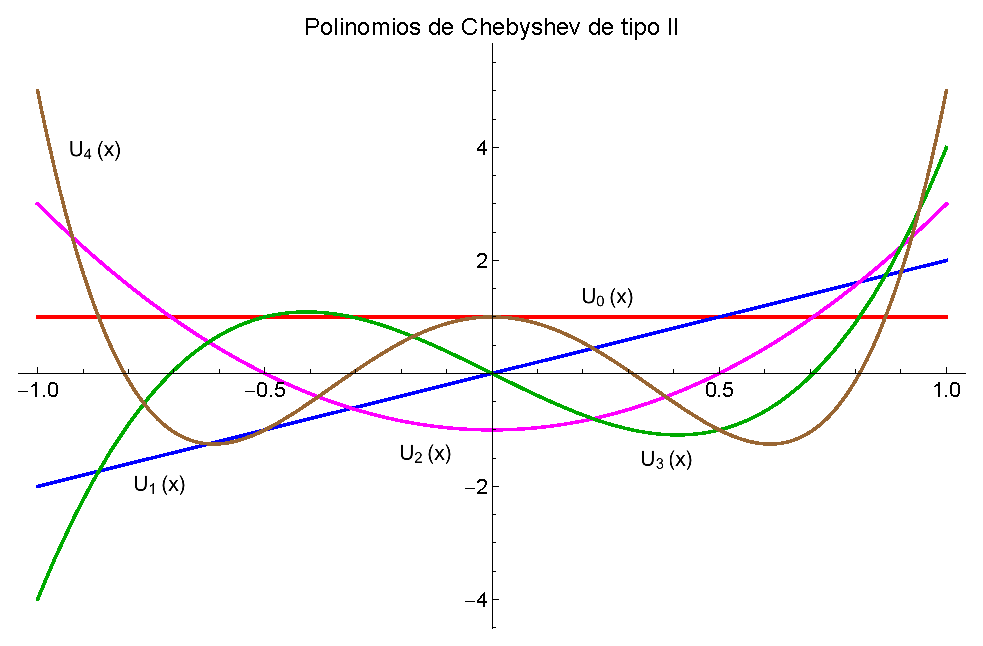
\includegraphics[scale=0.62]{Imagenes/Gram_Schmidt_Chebyshev_2.eps}
\end{figure}
\end{frame}

\end{document}